\documentclass[a4paper,11pt]{beamer}

\usepackage{préambule}
\usetikzlibrary{calc}

\begin{document}

\begin{frame}
	\begin{center}
		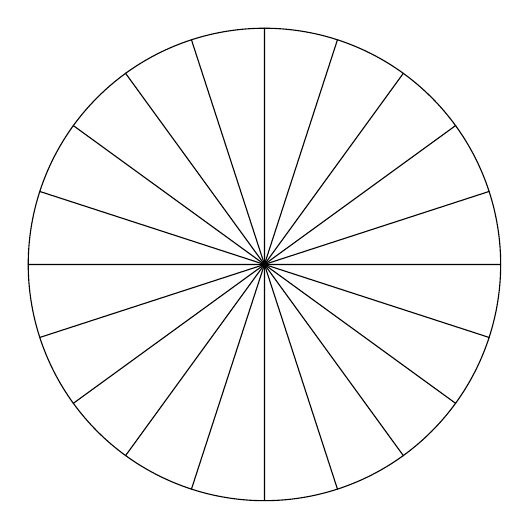
\begin{tikzpicture}
			\foreach \x in {1,...,20} {
					\draw[rotate=\x*18] (0,0) -- (3,0) arc[start angle=0, end angle=18,radius=3cm];
				}
		\end{tikzpicture}
	\end{center}
\end{frame}

\begin{frame}
	\begin{center}
		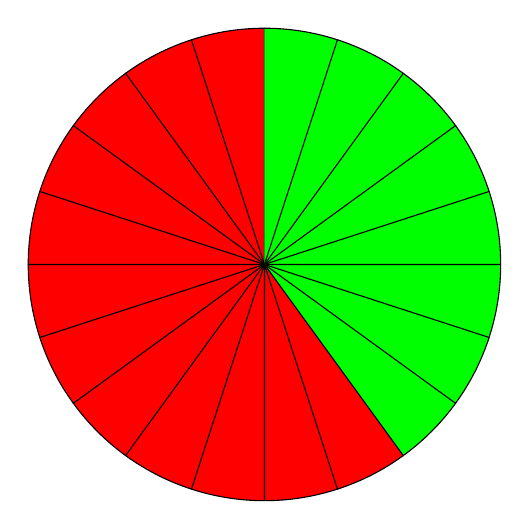
\begin{tikzpicture}
			\foreach \x in {1,...,12} {
					\draw[fill=red,rotate=\x*18+72] (0,0) -- (3,0) arc[start angle=0, end angle=18,radius=3cm];
				}
			\foreach \x in {13,...,20} {
					\draw[fill=green,rotate=\x*18+72] (0,0) -- (3,0) arc[start angle=0, end angle=18,radius=3cm];
				}
		\end{tikzpicture}
	\end{center}
\end{frame}

\begin{frame}
	\begin{center}
		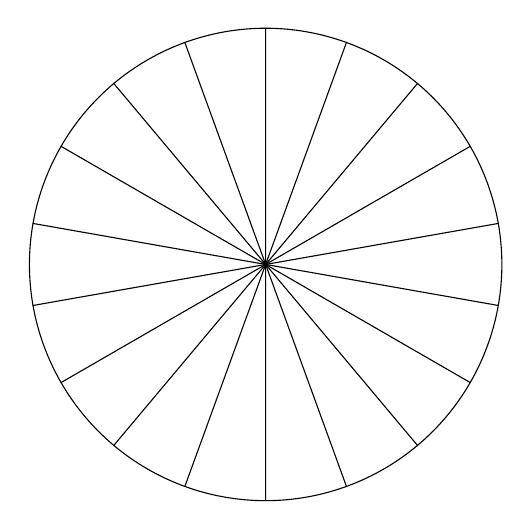
\begin{tikzpicture}
			\foreach \x in {1,...,18} {
					\draw[rotate=\x*20+10] (0,0) -- (3,0) arc[start angle=0, end angle=20,radius=3cm];
				}
		\end{tikzpicture}
	\end{center}
\end{frame}

\begin{frame}
	\begin{center}
		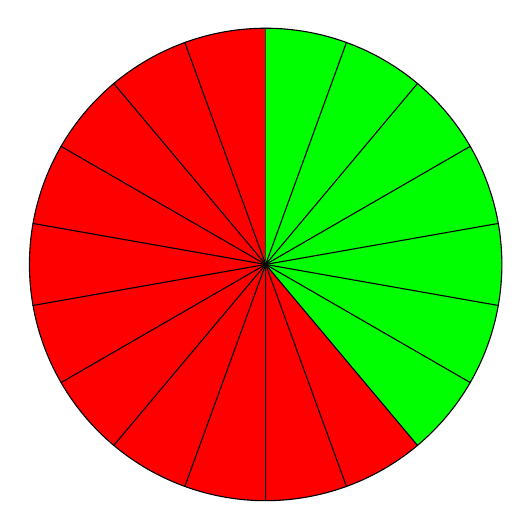
\begin{tikzpicture}
			\foreach \x in {1,...,11} {
					\draw[fill=red,rotate=\x*20+70] (0,0) -- (3,0) arc[start angle=0, end angle=20,radius=3cm];
				}
			\foreach \x in {12,...,18} {
					\draw[fill=green,rotate=\x*20+70] (0,0) -- (3,0) arc[start angle=0, end angle=20,radius=3cm];
				}
		\end{tikzpicture}
	\end{center}
\end{frame}

\begin{frame}
	\begin{center}
		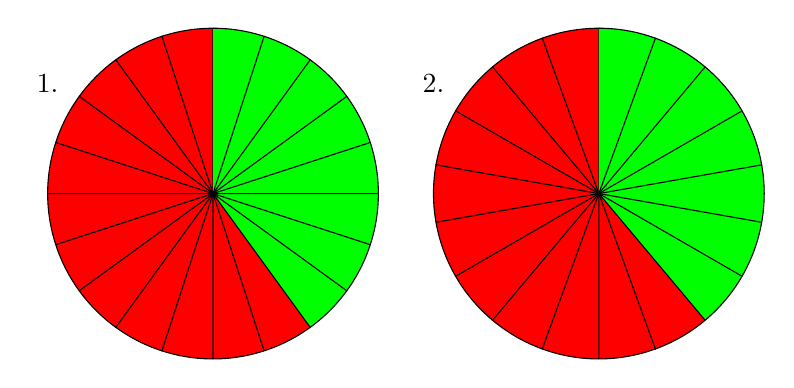
\begin{tikzpicture}[scale=0.7]
			\coordinate (A) at (0,0);
			\coordinate (B) at (7,0);

			\node at ($(A) + (-3,2)$) {1.};
			\node at ($(B) + (-3,2)$) {2.};
			\foreach \x in {1,...,12} {
					\draw[fill=red,rotate around={\x*18+72:(A)}] (A) -- ++(3,0) arc[start angle=0, end angle=18,radius=3cm];
				}
			\foreach \x in {13,...,20} {
					\draw[fill=green,rotate around={\x*18+72:(A)}] (A) -- ++(3,0) arc[start angle=0, end angle=18,radius=3cm];
				}

			\foreach \x in {1,...,11} {
					\draw[fill=red,rotate around={\x*20+70:(B)}] (B) -- ++(3,0) arc[start angle=0, end angle=20,radius=3cm];
				}
			\foreach \x in {12,...,18} {
					\draw[fill=green,rotate around={\x*20+70:(B)}] (B) -- ++(3,0) arc[start angle=0, end angle=20,radius=3cm];
				}
		\end{tikzpicture}
	\end{center}

	\begin{itemize}
		\item Quel est l'angle d'une part ? 1. ........° \hspace{1em} 2. ........°
		\item Quel est l'angle de la partie verte ?  1. ........° \hspace{1em} 2. ........°
	\end{itemize}
\end{frame}

\end{document}